\documentclass[]{article}
\usepackage{lmodern}
\usepackage{amssymb,amsmath}
\usepackage{ifxetex,ifluatex}
\usepackage{fixltx2e} % provides \textsubscript
\ifnum 0\ifxetex 1\fi\ifluatex 1\fi=0 % if pdftex
  \usepackage[T1]{fontenc}
  \usepackage[utf8]{inputenc}
\else % if luatex or xelatex
  \ifxetex
    \usepackage{mathspec}
  \else
    \usepackage{fontspec}
  \fi
  \defaultfontfeatures{Ligatures=TeX,Scale=MatchLowercase}
\fi
% use upquote if available, for straight quotes in verbatim environments
\IfFileExists{upquote.sty}{\usepackage{upquote}}{}
% use microtype if available
\IfFileExists{microtype.sty}{%
\usepackage{microtype}
\UseMicrotypeSet[protrusion]{basicmath} % disable protrusion for tt fonts
}{}
\usepackage[margin=1in]{geometry}
\usepackage{hyperref}
\hypersetup{unicode=true,
            pdftitle={Low level of covariance simulation},
            pdfauthor={Xuelong Wang},
            pdfborder={0 0 0},
            breaklinks=true}
\urlstyle{same}  % don't use monospace font for urls
\usepackage{graphicx,grffile}
\makeatletter
\def\maxwidth{\ifdim\Gin@nat@width>\linewidth\linewidth\else\Gin@nat@width\fi}
\def\maxheight{\ifdim\Gin@nat@height>\textheight\textheight\else\Gin@nat@height\fi}
\makeatother
% Scale images if necessary, so that they will not overflow the page
% margins by default, and it is still possible to overwrite the defaults
% using explicit options in \includegraphics[width, height, ...]{}
\setkeys{Gin}{width=\maxwidth,height=\maxheight,keepaspectratio}
\IfFileExists{parskip.sty}{%
\usepackage{parskip}
}{% else
\setlength{\parindent}{0pt}
\setlength{\parskip}{6pt plus 2pt minus 1pt}
}
\setlength{\emergencystretch}{3em}  % prevent overfull lines
\providecommand{\tightlist}{%
  \setlength{\itemsep}{0pt}\setlength{\parskip}{0pt}}
\setcounter{secnumdepth}{5}
% Redefines (sub)paragraphs to behave more like sections
\ifx\paragraph\undefined\else
\let\oldparagraph\paragraph
\renewcommand{\paragraph}[1]{\oldparagraph{#1}\mbox{}}
\fi
\ifx\subparagraph\undefined\else
\let\oldsubparagraph\subparagraph
\renewcommand{\subparagraph}[1]{\oldsubparagraph{#1}\mbox{}}
\fi

%%% Use protect on footnotes to avoid problems with footnotes in titles
\let\rmarkdownfootnote\footnote%
\def\footnote{\protect\rmarkdownfootnote}

%%% Change title format to be more compact
\usepackage{titling}

% Create subtitle command for use in maketitle
\providecommand{\subtitle}[1]{
  \posttitle{
    \begin{center}\large#1\end{center}
    }
}

\setlength{\droptitle}{-2em}

  \title{Low level of covariance simulation}
    \pretitle{\vspace{\droptitle}\centering\huge}
  \posttitle{\par}
    \author{Xuelong Wang}
    \preauthor{\centering\large\emph}
  \postauthor{\par}
      \predate{\centering\large\emph}
  \postdate{\par}
    \date{2019-08-23}

\usepackage{float,amsmath, bbm, siunitx, bm}
\usepackage{pdfpages}
\floatplacement{figure}{H}
\newcommand{\indep}{\rotatebox[origin=c]{90}{$\models$}}

\begin{document}
\maketitle

{
\setcounter{tocdepth}{2}
\tableofcontents
}
\section{Motivation}\label{motivation}

Based on the investigation of the covariance matrix patter of the PCBs
from 1999 - 2004, we found some patterns that appears among the
covariance matrix of PCBs from differert years. Besides, we also use the
historical data to estimate the covariance matrix, then use the sample
covariance matrix to decorrelate the PCBs for each year. For most years,
the decorrelation procedure can reduce the correlation, e.g 1999-2001,
but there are some years which the correlations still are high after
decorrelation, e.g 2005-2006.

Since we are trying to borrow information of historical dataset, the
decorrelated data will probably not be perfert uncorrelted. In other
words, we will end up with data with low correlations among their
coveriates. So the goal of this report is to see if the GCTA and
EigenPrism method could work well under the low correlation setup.

\section{setup}\label{setup}

\subsection{Sample covariance matrix}\label{sample-covariance-matrix}

I use two different sample covariane matrices: 1999-2001 and 2007 -2008.

\begin{figure}
\centering
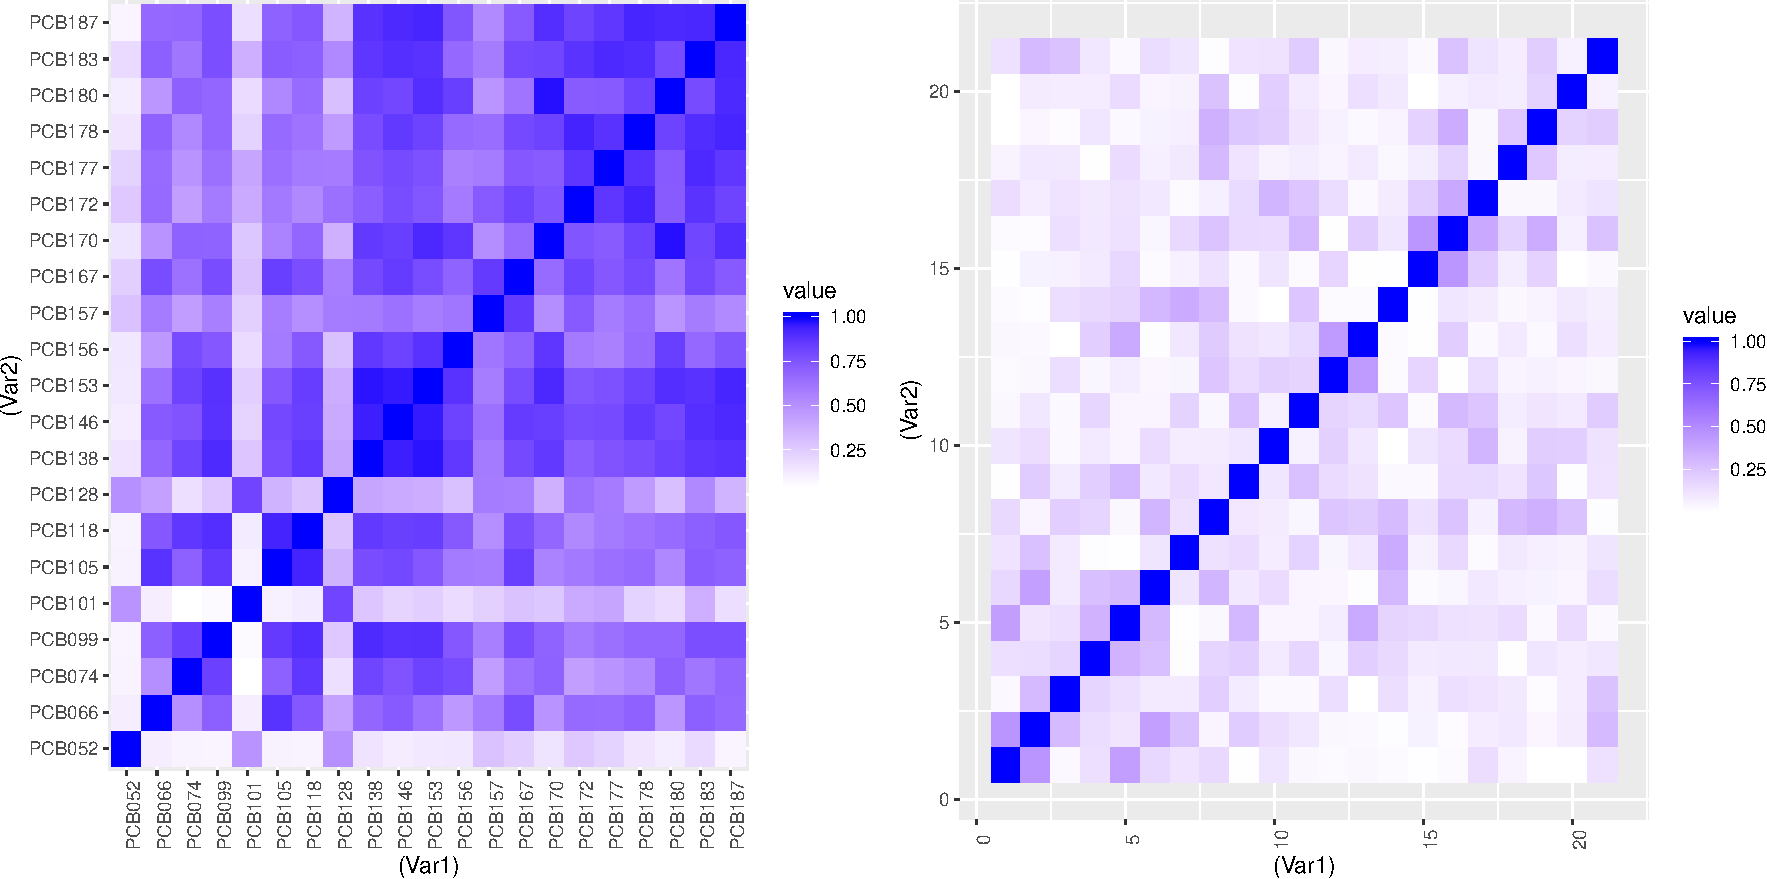
\includegraphics{Low_levels_covariance_files/figure-latex/unnamed-chunk-2-1.pdf}
\caption{1999-2000}
\end{figure}

\begin{figure}
\centering
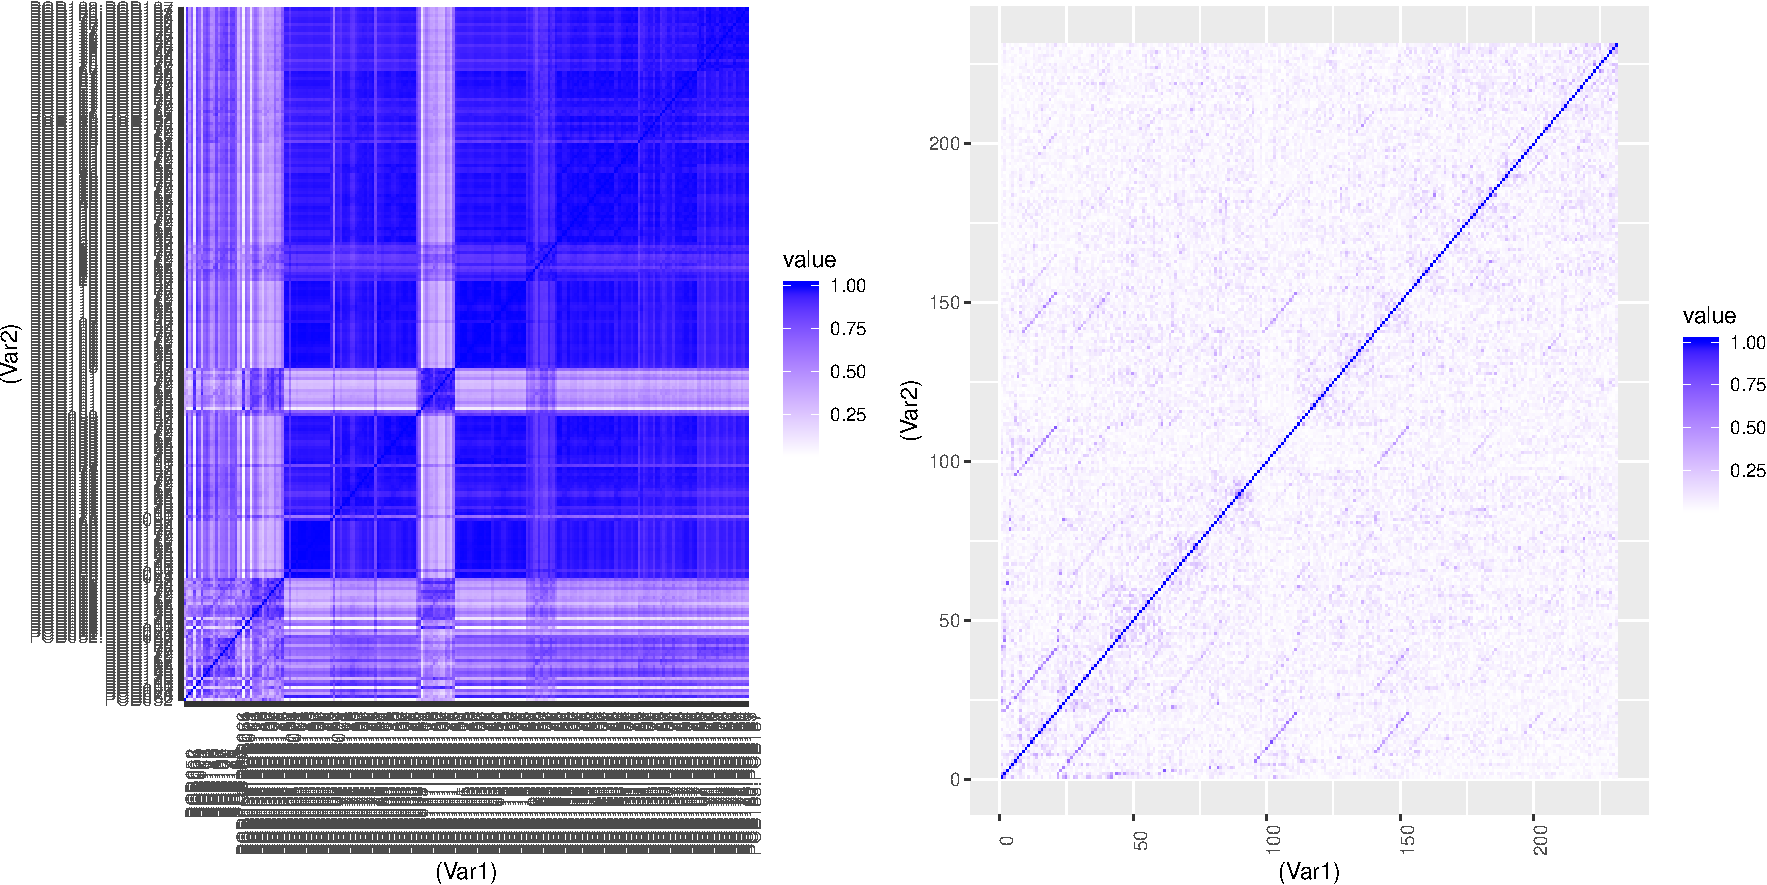
\includegraphics{Low_levels_covariance_files/figure-latex/unnamed-chunk-3-1.pdf}
\caption{Combined main and interaction 1999-2000}
\end{figure}

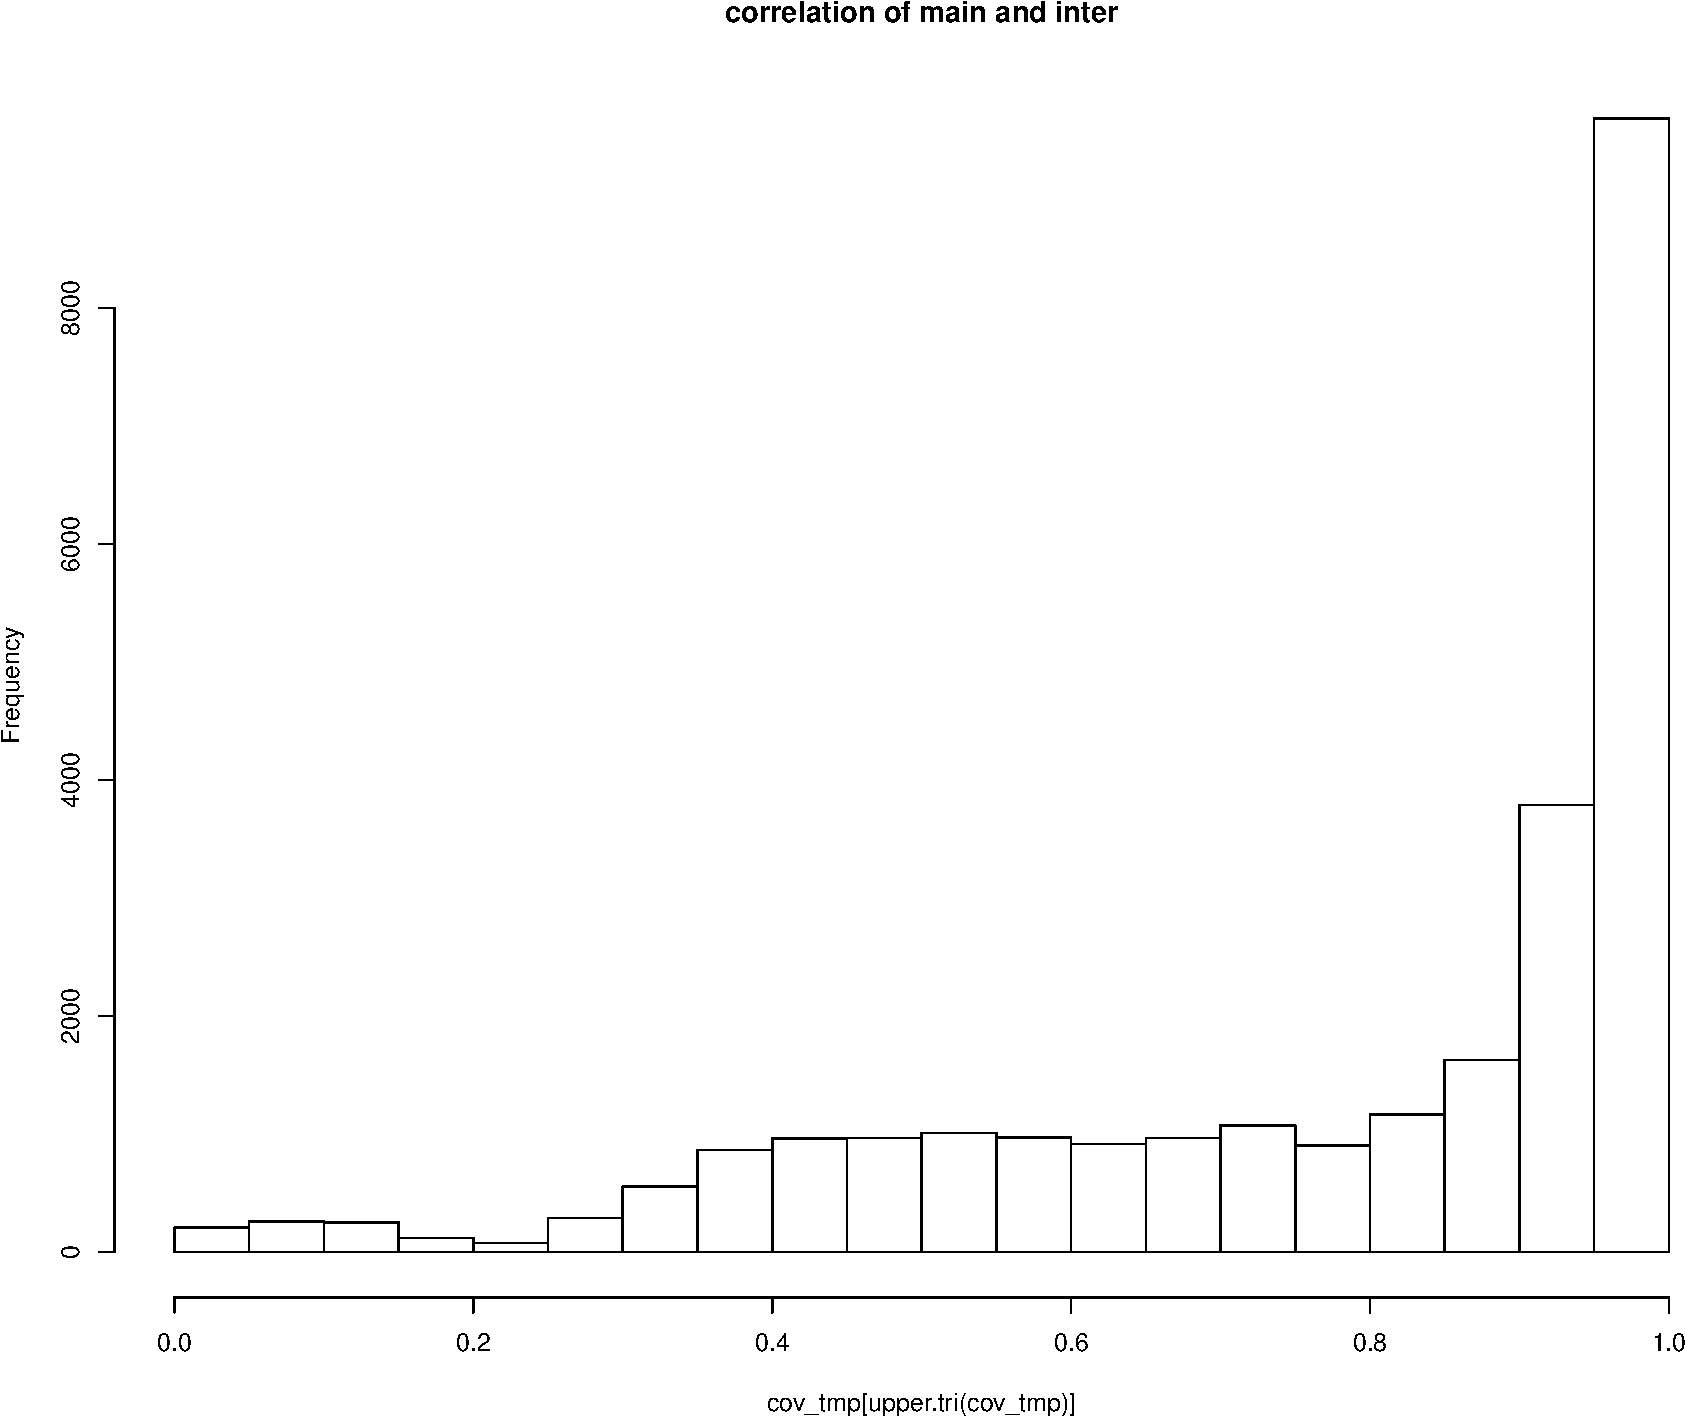
\includegraphics{Low_levels_covariance_files/figure-latex/unnamed-chunk-4-1.pdf}

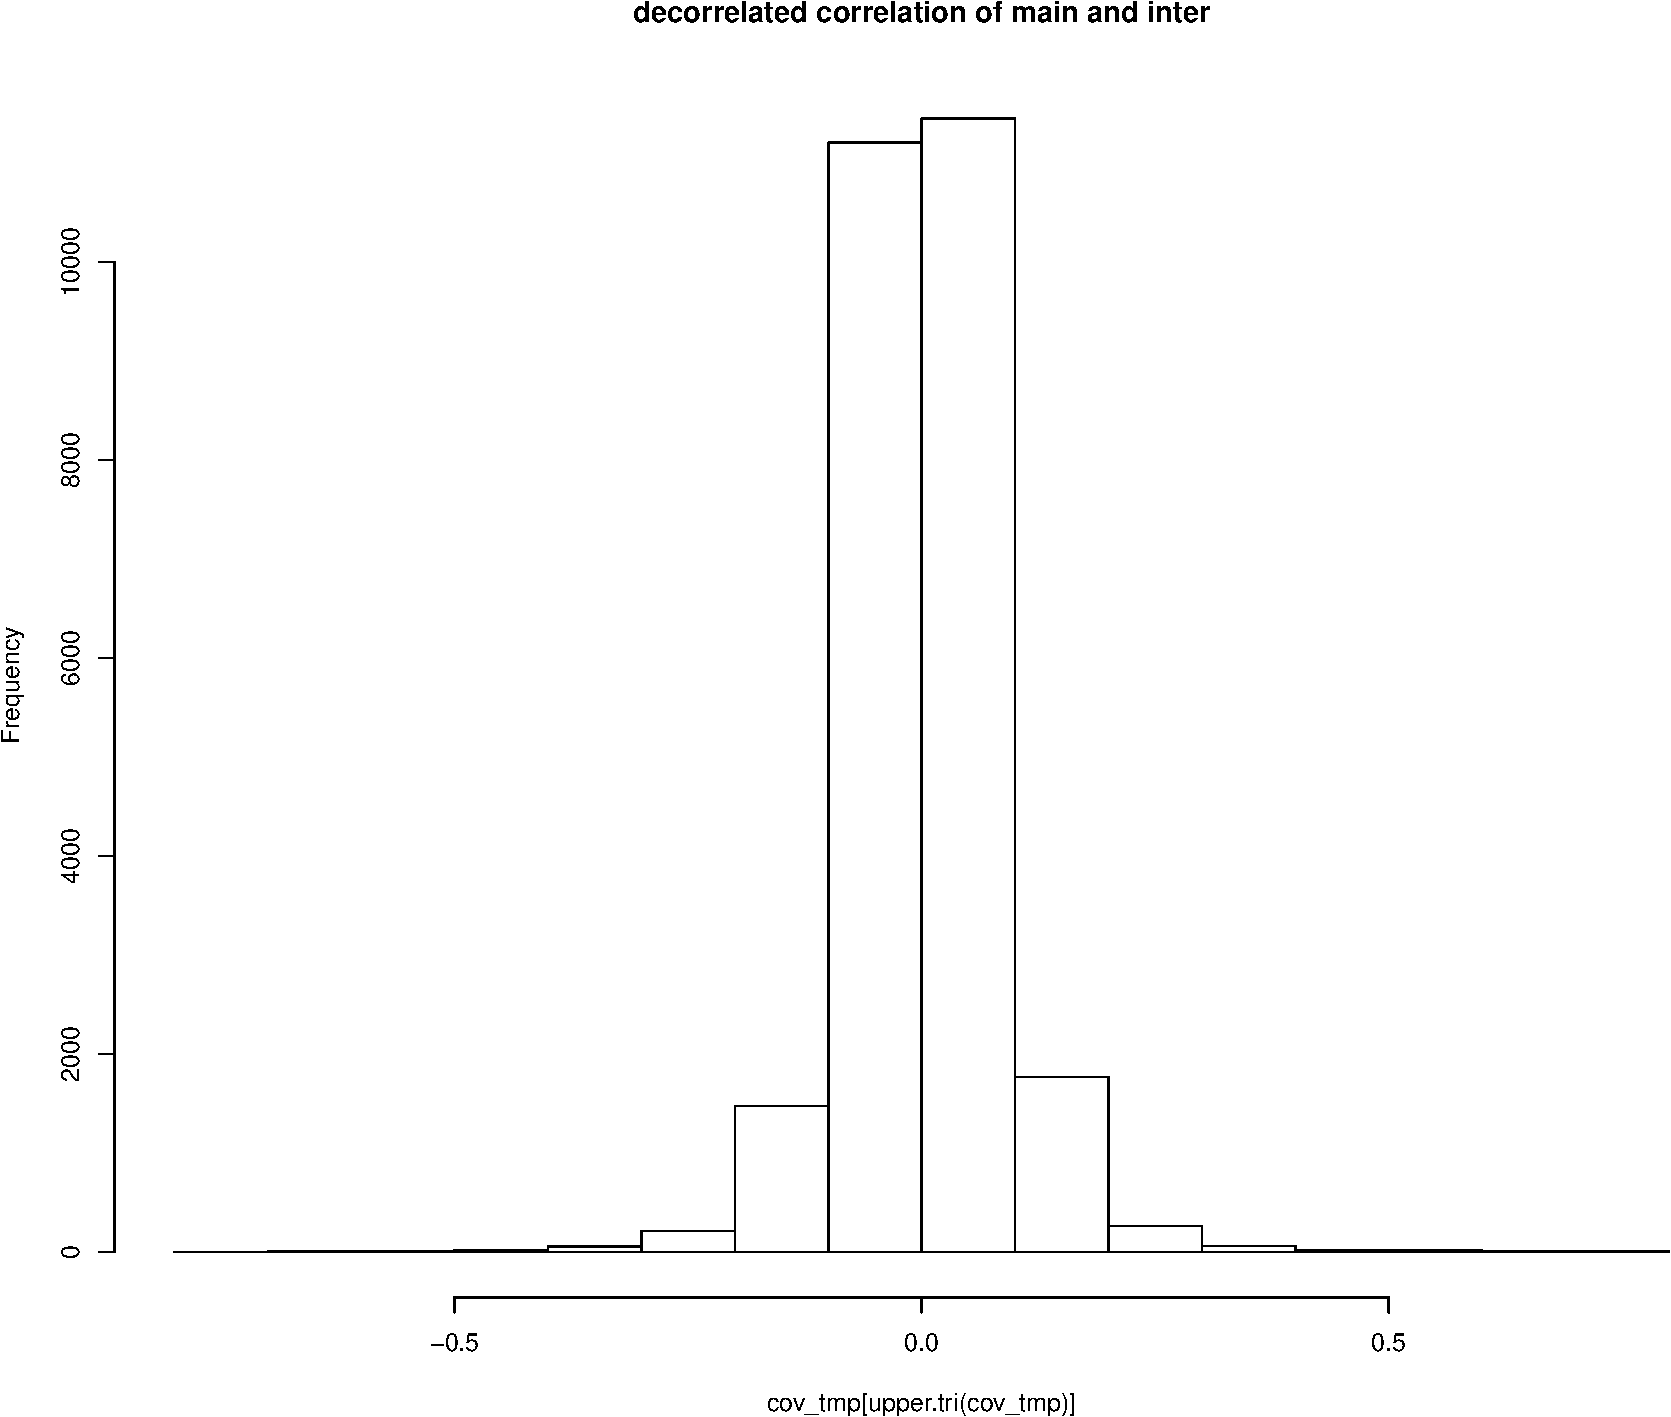
\includegraphics{Low_levels_covariance_files/figure-latex/unnamed-chunk-5-1.pdf}

\begin{figure}
\centering
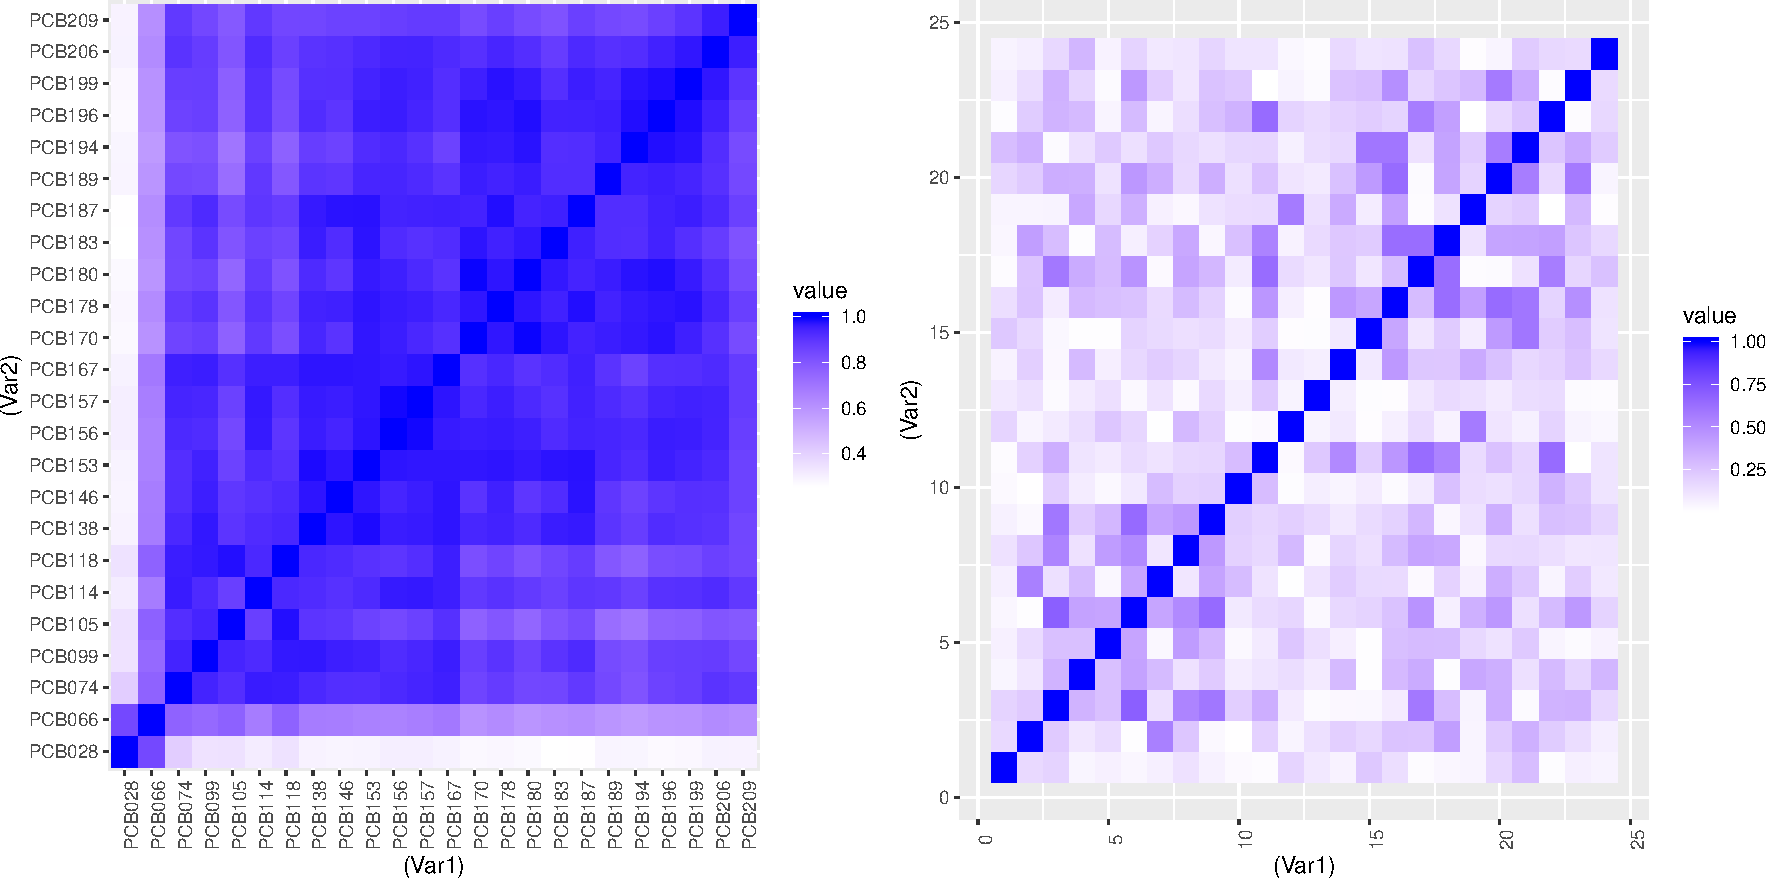
\includegraphics{Low_levels_covariance_files/figure-latex/unnamed-chunk-7-1.pdf}
\caption{2005-2006}
\end{figure}

\begin{figure}
\centering
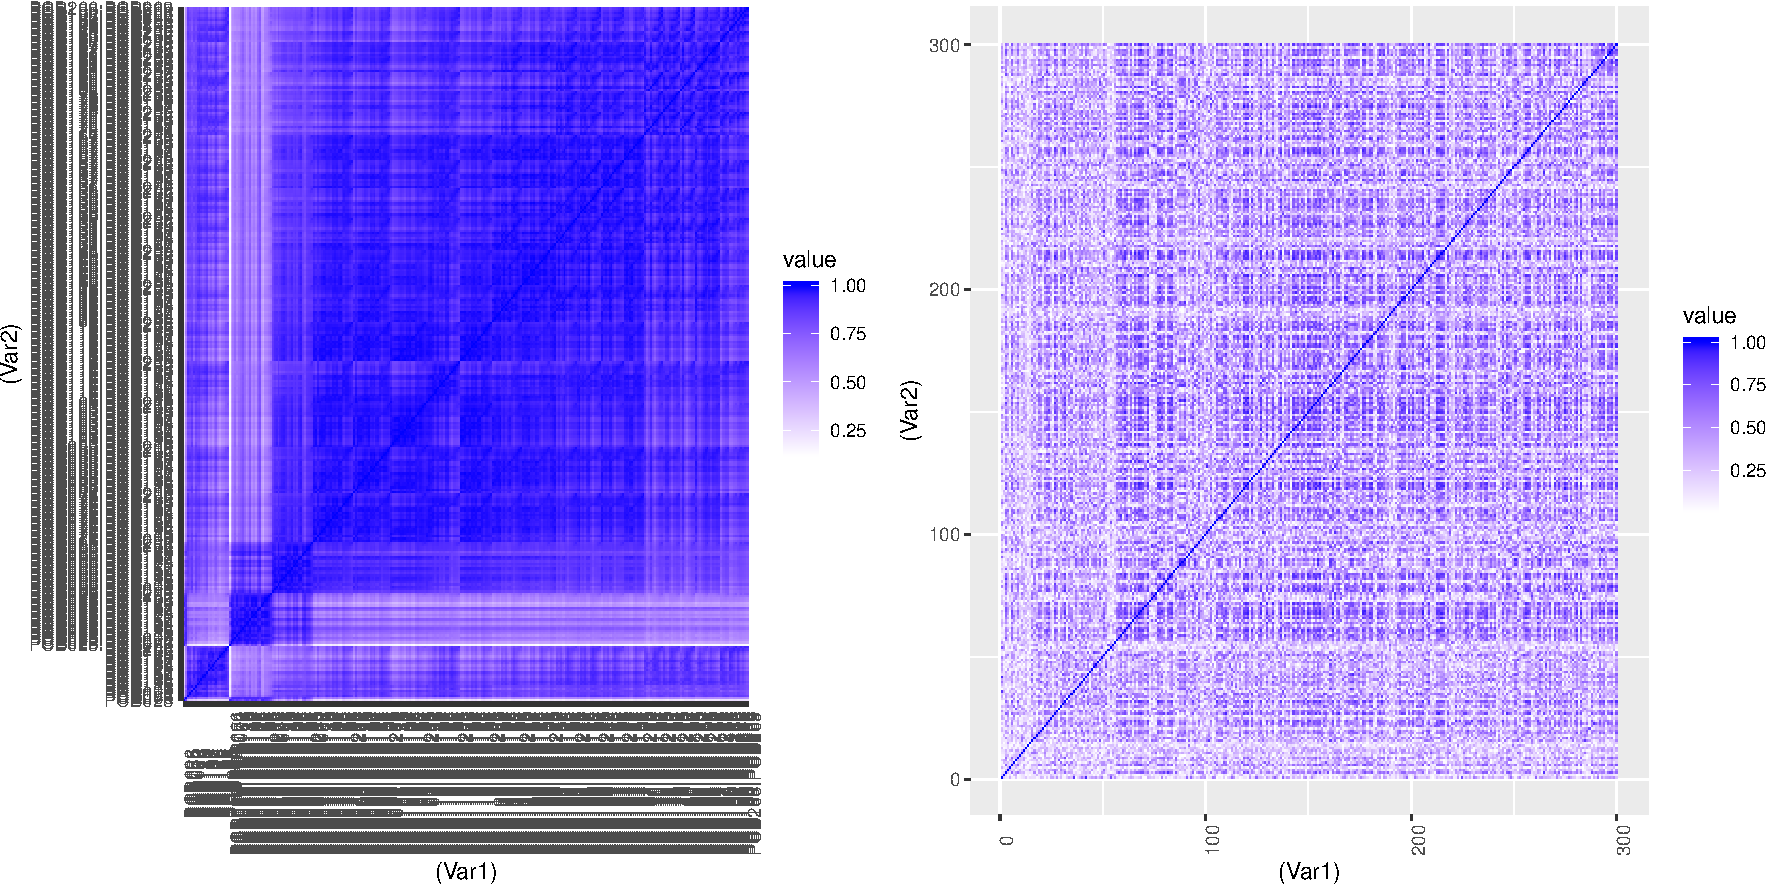
\includegraphics{Low_levels_covariance_files/figure-latex/unnamed-chunk-8-1.pdf}
\caption{Combined main and interaction 2005-2006}
\end{figure}

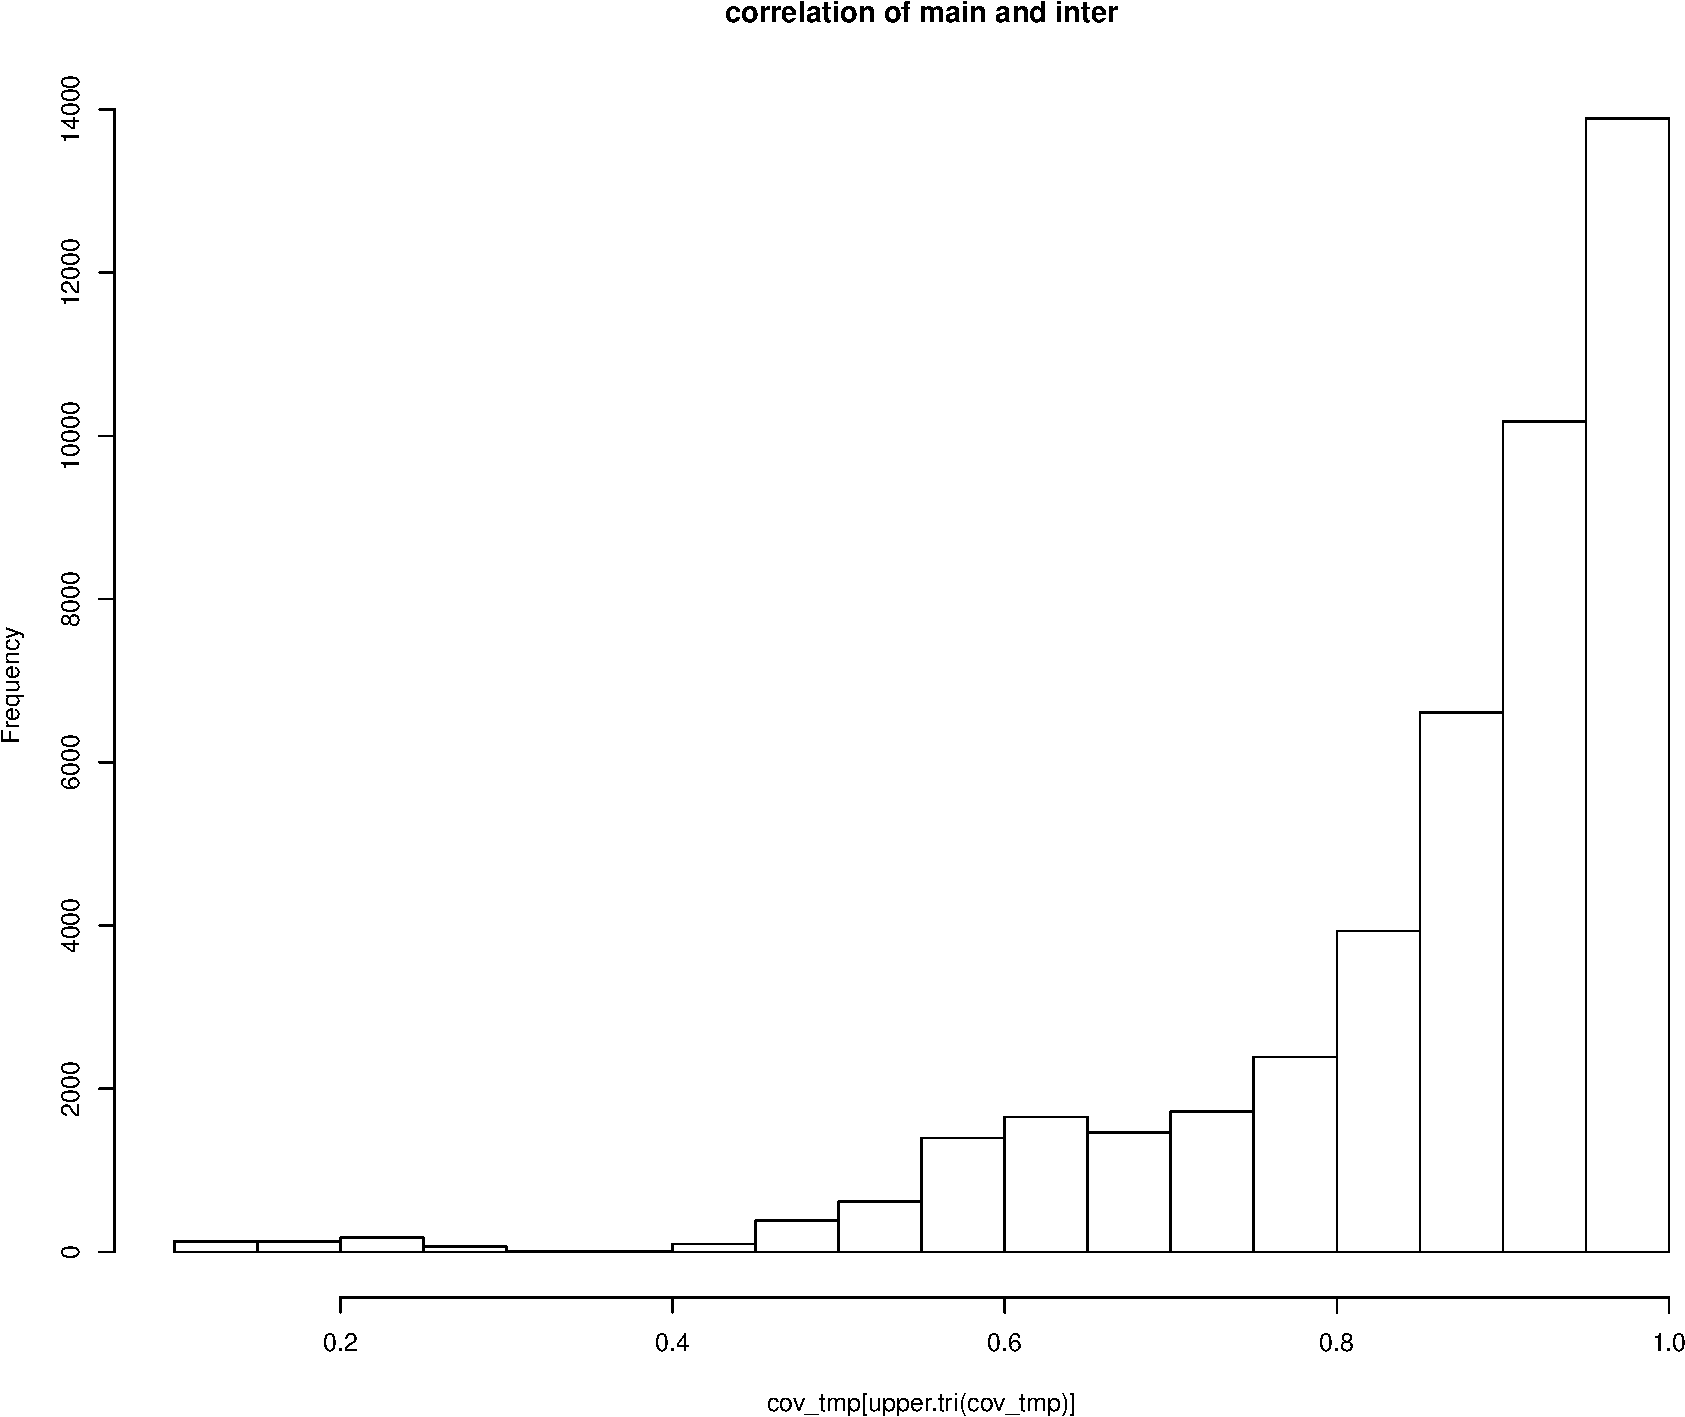
\includegraphics{Low_levels_covariance_files/figure-latex/unnamed-chunk-9-1.pdf}

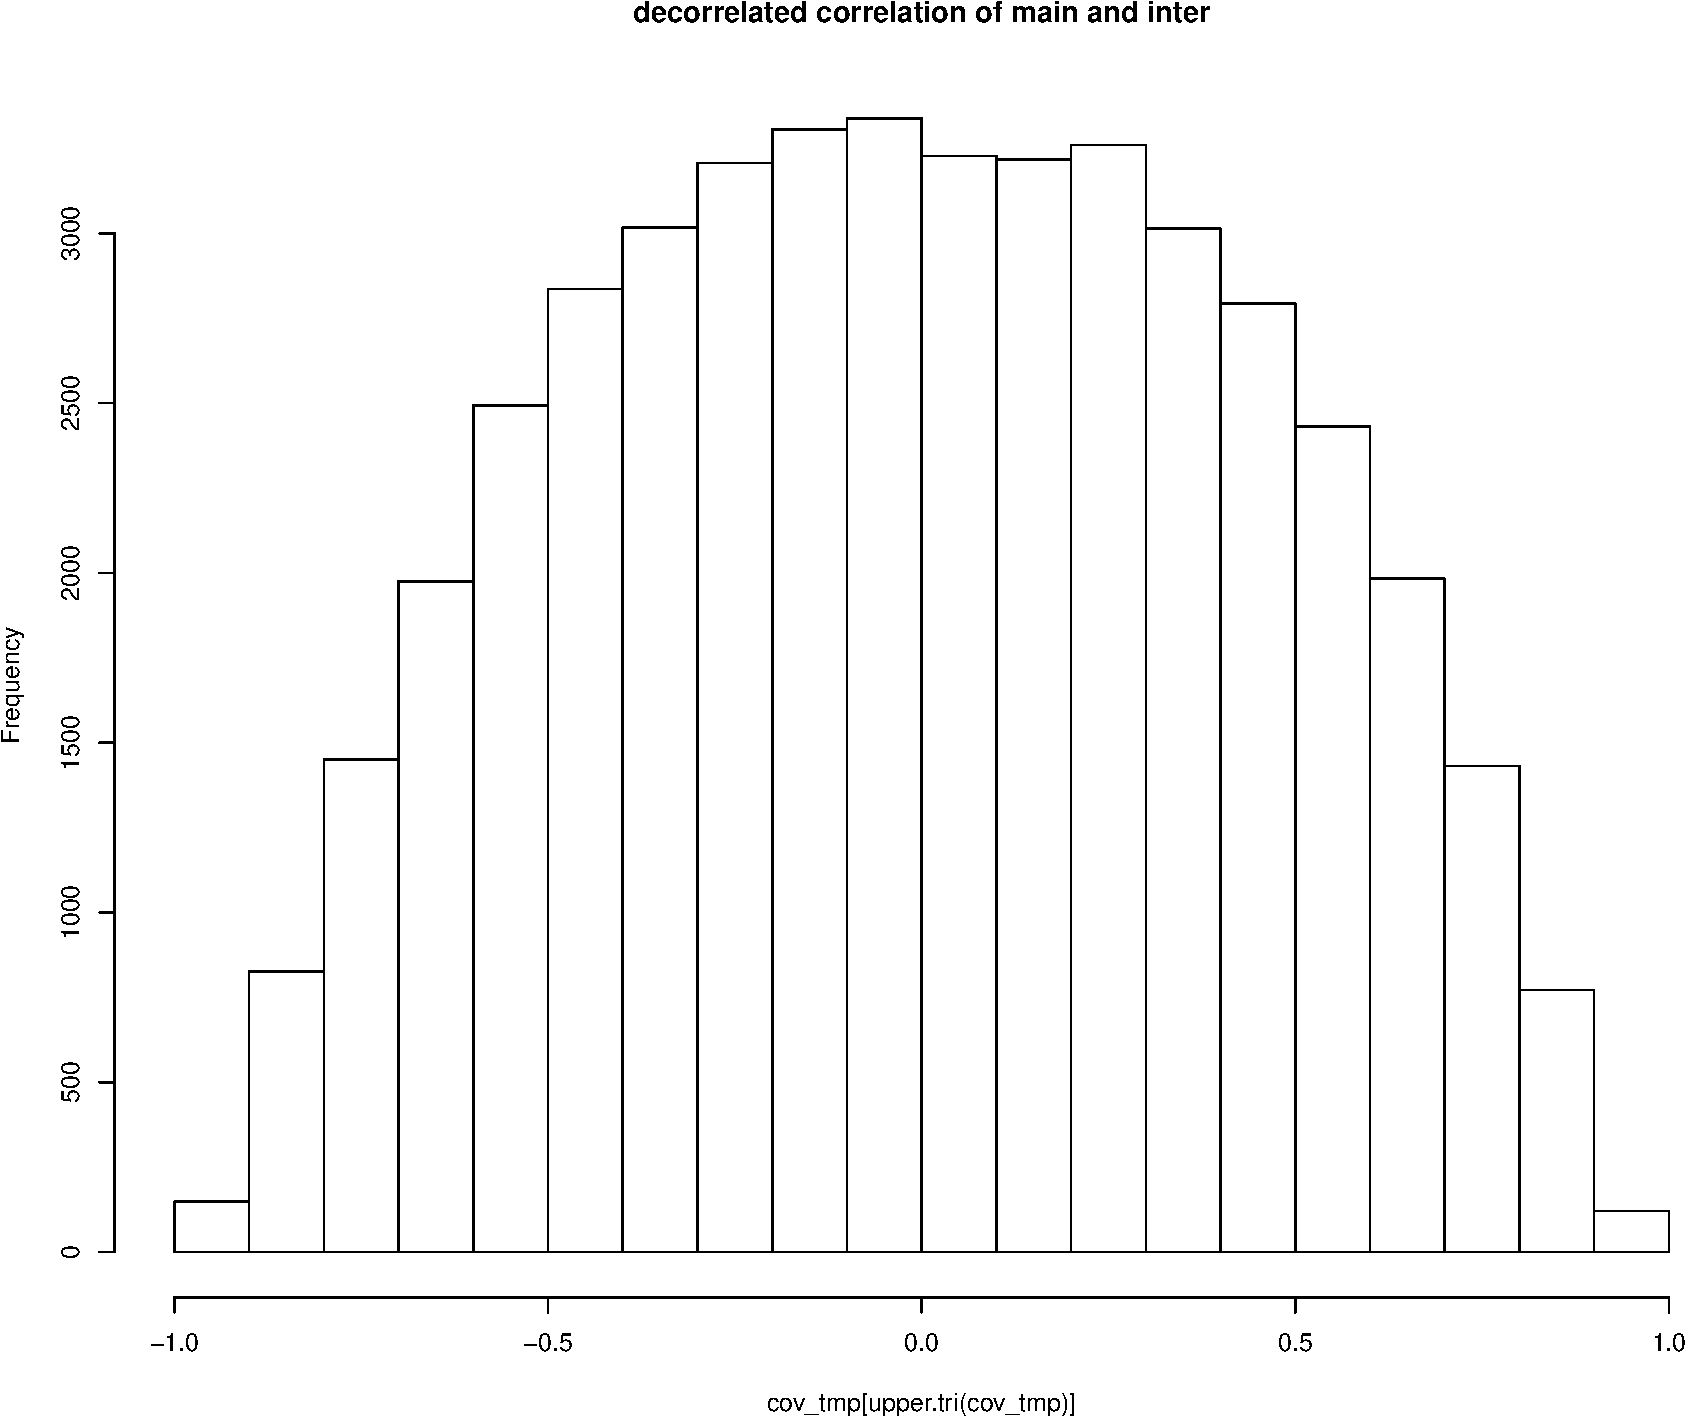
\includegraphics{Low_levels_covariance_files/figure-latex/unnamed-chunk-10-1.pdf}

\newpage

\subsection{Simulation setup}\label{simulation-setup}

\begin{enumerate}
\def\labelenumi{\arabic{enumi}.}
\tightlist
\item
  p = 231 for 1999 or 300 for 2005\\
\item
  \(n \in \{100, 150, p\}\)\\
\item
  the simulated covariates will follow Normal or Chi with df = 1\\
\item
  Variance estimation method will be GCTA and EigenPrism method\\
\item
  Iteration time is 100
\end{enumerate}

\section{Result}\label{result}

\subsection{1999}\label{section}

\begin{verbatim}
      n  MSE est_var est_mean     method target var_main_effect decor
 1: 100 19.6    18.9     10.9 EigenPrism   main              10 FALSE
 2: 150  8.7     8.7     10.2 EigenPrism   main              10 FALSE
 3: 231  5.5     5.5     10.1 EigenPrism   main              10 FALSE
 4: 100 21.3    21.4     10.3       GCTA   main              10 FALSE
 5: 150  9.3     9.4     10.1       GCTA   main              10 FALSE
 6: 231  5.0     5.1     10.0       GCTA   main              10 FALSE
 7: 100 20.6    20.6     10.4 EigenPrism   main              10 FALSE
 8: 150 10.4    10.4      9.7 EigenPrism   main              10 FALSE
 9: 231  5.3     5.2     10.4 EigenPrism   main              10 FALSE
10: 100 20.7    21.0     10.0       GCTA   main              10 FALSE
11: 150 10.9    10.6      9.4       GCTA   main              10 FALSE
12: 231  4.8     4.7     10.4       GCTA   main              10 FALSE
    x_dist
 1:    chi
 2:    chi
 3:    chi
 4:    chi
 5:    chi
 6:    chi
 7: normal
 8: normal
 9: normal
10: normal
11: normal
12: normal
\end{verbatim}

\subsection{2005}\label{section-1}

\begin{verbatim}
      n  MSE est_var est_mean     method target var_main_effect decor
 1: 100 16.4    15.8     10.9 EigenPrism   main              10 FALSE
 2: 150 13.3    11.6     11.3 EigenPrism   main              10 FALSE
 3: 300  4.5     4.6      9.9 EigenPrism   main              10 FALSE
 4: 100 12.3    11.2     11.1       GCTA   main              10 FALSE
 5: 150 11.0     7.7     11.8       GCTA   main              10 FALSE
 6: 300  3.7     3.0     10.9       GCTA   main              10 FALSE
 7: 100 15.1    13.6     11.3 EigenPrism   main              10 FALSE
 8: 150 11.4    10.6     11.0 EigenPrism   main              10 FALSE
 9: 300  6.7     6.7     10.3 EigenPrism   main              10 FALSE
10: 100 12.1    10.2     11.4       GCTA   main              10 FALSE
11: 150  9.4     7.2     11.5       GCTA   main              10 FALSE
12: 300  4.4     3.4     11.0       GCTA   main              10 FALSE
    x_dist
 1:    chi
 2:    chi
 3:    chi
 4:    chi
 5:    chi
 6:    chi
 7: normal
 8: normal
 9: normal
10: normal
11: normal
12: normal
\end{verbatim}


\end{document}
